%%%%%%%%%%%%%%%%%%%%%%%%%%%%%%%%%%%%%%%%%
% Journal Article
% LaTeX Template
% Version 1.4 (15/5/16)
%
% This template has been downloaded from:
% http://www.LaTeXTemplates.com
%
% Original author:
% Frits Wenneker (http://www.howtotex.com) with extensive modifications by
% Vel (vel@LaTeXTemplates.com)
%
% License:
% CC BY-NC-SA 3.0 (http://creativecommons.org/licenses/by-nc-sa/3.0/)
%
%%%%%%%%%%%%%%%%%%%%%%%%%%%%%%%%%%%%%%%%%

%----------------------------------------------------------------------------------------
%	PACKAGES AND OTHER DOCUMENT CONFIGURATIONS
%----------------------------------------------------------------------------------------

\documentclass[twoside]{article}

\usepackage{blindtext} % Package to generate dummy text throughout this template 

\usepackage[sc]{mathpazo} % Use the Palatino font
\usepackage[T1]{fontenc} % Use 8-bit encoding that has 256 glyphs
\linespread{1.05} % Line spacing - Palatino needs more space between lines
\usepackage{microtype} % Slightly tweak font spacing for aesthetics

\usepackage[english]{babel} % Language hyphenation and typographical rules

\usepackage[hmarginratio=1:1,top=32mm,columnsep=20pt]{geometry} % Document margins
\usepackage[hang, small,labelfont=bf,up,textfont=it,up]{caption} % Custom captions under/above floats in tables or figures
\usepackage{booktabs} % Horizontal rules in tables

\usepackage{lettrine} % The lettrine is the first enlarged letter at the beginning of the text

\usepackage{enumitem} % Customized lists
\setlist[itemize]{noitemsep} % Make itemize lists more compact

\usepackage{abstract} % Allows abstract customization
\renewcommand{\abstractnamefont}{\normalfont\bfseries} % Set the "Abstract" text to bold
\renewcommand{\abstracttextfont}{\normalfont\small\itshape} % Set the abstract itself to small italic text

\usepackage{titlesec} % Allows customization of titles
\renewcommand\thesection{\Roman{section}} % Roman numerals for the sections
\renewcommand\thesubsection{\roman{subsection}} % roman numerals for subsections
\titleformat{\section}[block]{\large\scshape\centering}{\thesection.}{1em}{} % Change the look of the section titles
\titleformat{\subsection}[block]{\large}{\thesubsection.}{1em}{} % Change the look of the section titles

\usepackage{fancyhdr} % Headers and footers
\pagestyle{fancy} % All pages have headers and footers
\fancyhead{} % Blank out the default header
\fancyfoot{} % Blank out the default footer
\fancyhead[C]{Running title $\bullet$ May 2016 $\bullet$ Vol. XXI, No. 1} % Custom header text
\fancyfoot[RO,LE]{\thepage} % Custom footer text

\usepackage{titling} % Customizing the title section

% My packages (not template)
\usepackage{hyperref} % For hyperlinks in the PDF
%\usepackage{amsmath}
\usepackage{amssymb}
\usepackage{authblk}
\usepackage{graphicx}
\graphicspath{ {figures_report/} }

% From mortens LaTex file:
\usepackage{amsfonts, amssymb, amsmath}
\newcommand{\md}{\mathrm{d}}
\newcommand{\e}[1]{\times 10^{#1}}
\newcommand{\bra}[1]{\langle #1 |}
\newcommand{\ket}[1]{| #1 \rangle}
\newcommand{\braket}[2]{\langle #1 | #2 \rangle}
\renewcommand{\vec}[1]{\mathbf{#1}}
\newcommand{\gvec}[1]{\boldsymbol{#1}}
\newcommand{\dr}{\, \mathrm d^3 \vec r}
\newcommand{\dk}{\, \mathrm d^3 \vec k}

%----------------------------------------------------------------------------------------
%	TITLE SECTION
%----------------------------------------------------------------------------------------

\setlength{\droptitle}{-4\baselineskip} % Move the title up

\pretitle{\begin{center}\Huge\bfseries} % Article title formatting
\posttitle{\end{center}} % Article title closing formatting
\title{Building a Shell Model Code: The Pairing Model and the sd-Shell (and comparing results with NuShellX)} % Article title


\author[1]{ \textsc{Gianluca Salvioni}}
\author[2]{ \textsc{Ina K. B. Kullmann}}
\author[3]{ \textsc{Matthew Shelley}}
\author[4]{ \textsc{Gilho Ahn}}


\affil[1]{Department of FILL IN, \LaTeX\ University,  {\textit {\href{mailto:youremail@edu.com}{youremail@edu.com} }}}

\affil[2]{Department of Physics, University of Oslo,  {\textit {\ \href{mailto:i.k.b.kullmann@fys.uio.no}{i.k.b.kullmann@fys.uio.no} }}}

\affil[3] {Department of FILL IN, \LaTeX\ University, \textit {\href{mailto:youremail@edu.com}{youremail@edu.com} }}

\affil[4] {Department of FILL IN, \LaTeX\ University, \textit {\href{mailto:youremail@edu.com}{youremail@edu.com} }}


% another way of doing the authors:
%\author{%
%\textsc{Gianluca Salvioni, Matthew Shelley, Gilho Ahn}\thanks{A thank you} \\[1ex]
%\normalsize University of Oslo \\ % Your institution
%\normalsize \href{mailto:i.k.b.kullmann@fys.uio.no}{i.k.b.kullmann@fys.uio.no} % Your email address
%\and % Uncomment if 2 authors are required, duplicate these 4 lines if more
%\textsc{Ina K. B. Kullmann}\thanks{Corresponding author} \\[1ex] % Second author's name
%\normalsize University of Oslo \\ % Your institution
%\normalsize \href{mailto:i.k.b.kullmann@fys.uio.no}{i.k.b.kullmann@fys.uio.no} % Your email address
%}



\date{\today} % Leave empty to omit a date

\renewcommand{\maketitlehookd}{%
\begin{abstract}

We have first implemented the pairing model which have a analytical solution (to benchmark the code). Then implemented the sd shell ---> more general shell-model program that allows you to study general nuclear structure problems.

developing our own shell-model code that can perform shell-model studies of the oxygen isotopes using standard effective interactions (provided by us) using as example the 1s0d shell as model space.

We have also used the NushellX code in order to perform more advanced shell-model studies and compare the results obtained with your own shell-model code to those of NushellX

and found that.....results...

\end{abstract}
}

%----------------------------------------------------------------------------------------

\begin{document}

% Print the title
\maketitle

%----------------------------------------------------------------------------------------
%	ARTICLE CONTENTS
%----------------------------------------------------------------------------------------

\section{Introduction}

\lettrine[nindent=0em,lines=3]{L} orem ipsum dolor sit amet, consectetur adipiscing elit.
\blindtext % Dummy text

\blindtext % Dummy text

%------------------------------------------------

\section{Theory}

%say something general here?

\subsection{Exact results: The Pairing Model}

The pairing model is one of a few systems that has a simple analytic solution. It is therefore very useful to use this model to check that the numerical solution matches the analytic solution while developing the code. %From project text: It is a model which to a large extent mimicks some central features of atomic nuclei, certain atoms and systems which exhibit superfluiditity or superconductivity. Pairing plays a central role in nuclear physics, in particular, for identical particles it makes up large fractions of the correlations among particles.

The pairing problem consists of a system where the fermions combines together in pairs of two, one with spin up and one with spin down. This model does not allow so-called 'breaking of pairs' meaning that the pairs of particles always will be coupled together. An excitation must excite two particles at the same time. 

Mathematically the pairing model can be described by a simplified Hamiltonian consisting of a unperturbed one-body operator $H^0$ and a pertubation so-called 'pairing interaction term' $H^I$. We will limit ourselves to at most two-body interactions so that we can write the operators as:

\begin{equation}
\hat H_0 = \xi \sum_{p,\sigma} (p-1) \hat a_{p\sigma}^\dagger \hat a_{p\sigma},
\label{eq:H_0}
\end{equation}

\begin{equation}
\hat V = -\frac{1}{2} g \sum_{p,q} \hat a_{p+}^\dagger \hat a_{p-}^\dagger \hat a_{q-} \hat a_{q+} ,\label{eq:V}
\end{equation}
so that the full Hamiltonian is given by the sum of the unperturbed term and the interacting part $\hat H = \hat H_0 + \hat V$. The fermion creation and annihilation operators are given by $\hat a_{p}^\dagger$ and $\hat a_{q}$ respectively and $pqrs$ represent all possible single-particle quantum numbers. To simplify the expressions we set the spacing between successive single-particle states given by $\xi=1$.

We will let the single-particle states$\vert p \rangle$ be eigenfunctions of the one-particle operator $\hat{h}_0$. The above Hamiltonian acts in turn on various many-body Slater determinants constructed from the single-basis defined by the one-body operator $\hat{h}_0$ .


The two-body operator $\hat{V}$ consists of one term:
\begin{equation}
\langle q_+ q_- \vert \hat{V} \vert s_+s_- \rangle = -g
\end{equation}
representing the pairing contribution with (for simplicity) constant strength $g$. The labeling requires that for a given matrix element $\langle pq \vert \hat{V} \vert rs \rangle$ the states $p$ and $q$ (or $r$ and $s$) must have opposite spin ($\sigma=\pm 1$)

It can be shown that the unperturbed Hamiltonian $\hat{H}_0$ and $\hat{V}$ commute with the spin projection $\hat{S}_z$ and the total spin $\hat{S}^2$. This allows us to block-diagonalize the full Hamiltonian. For the pairing case we have assumed that $S = 0$ giving the so-called 'no-broken pair' case.





\paragraph{Constructing the Hamiltonian matrix}

As an exact analytic solution we chose a system consisting of only four particles with a single-particle space consisting of only the four lowest levels $p = 1, 2, 3, 4$. In our system every level $p$ contains two particles, one with spin up and one with spin down. The goal is to set up all possible Slater determinants and the Hamiltonian matrix using second quantization and find all eigenvalues by diagonalizing the Hamiltonian matrix.

We construct the basis:
\[ \ket{\Phi_0} = \begin{pmatrix} 1 \\ 0 \\ 0 \\ 0 \\ 0 \\ 0 \end{pmatrix}, \quad
\ket{\Phi_1} = \begin{pmatrix} 0 \\ 1 \\ 0 \\ 0 \\ 0 \\ 0 \end{pmatrix}, \quad \cdots \quad
\ket{\Phi_5} = \begin{pmatrix} 0 \\ 0 \\ 0 \\ 0 \\ 0 \\ 1 \end{pmatrix}, \]

where
\begin{align*}
\ket{\Phi_0} &= \hat a_{2+}^\dagger \hat a_{2-}^\dagger \hat a_{1+}^\dagger \hat a_{1-}^\dagger \ket{0} = \hat P_2^+ \hat P_1^+ \ket{0}, \\
%
\ket{\Phi_1} &= \hat P_3^+ \hat P_1^+ \ket{0}, \\
%
\ket{\Phi_2} &= \hat P_4^+ \hat P_1^+ \ket{0}, \\
%
\ket{\Phi_3} &= \hat P_3^+ \hat P_2^+ \ket{0}, \\
%
\ket{\Phi_4} &= \hat P_4^+ \hat P_2^+ \ket{0}, \\
%
\ket{\Phi_5} &= \hat P_4^+ \hat P_3^+ \ket{0}. \\
\end{align*}

Given the above Slater determinants  we can now compute the matrix elements $\bra{\Phi_i} \hat H \ket{\Phi_j}$ using the Hamiltonian of Eq.~\eqref{eq:H_0}. The one-body operator acts only on the diagonal and results in terms proportional with $(p − 1)$. The interaction will excite or deexcite a pair of particles from level $q$ to level $p$. Using this it is easy to see that the Hamilotnian matrix becomes: (REWRITE THIS PARAGRAPH,  ALL COPY)

\begin{equation}
\hat H = \begin{pmatrix}
2 - g & -g/2 & -g/2 & -g/2 & -g/2 & 0 \\
-g/2 & 4- g & -g/2 & -g/2 & 0 & -g/2 \\
-g/2 & -g/2 & 6 -g & 0 & -g/2 & -g/2 \\
-g/2 & -g/2 & 0 & 6 -g & -g/2 & -g/2 \\
-g/2 & 0 & -g/2 & -g/2 & 8 - g & -g/2 \\
0 & -g/2 & -g/2 & -g/2 & -g/2 & 10 - g \\
\end{pmatrix} .
\label{eq: analytic_H_matrix} 
\end{equation}

For a given $g$ this matrix can be used as the analytic result to compare with the output from the shell model code for the pairing case. ....%These results will serve as a benchmark for the construction of our shell-model program. We refer to this as the exact results. 




\section{Building the shell model code}

develop a code which sets up the above Hamiltonian matrices for two and four particles in 2 and 4 single-particles states (the same as what you did in exercises b) and c) and obtain the eigenvalues.

What did we choose?
\begin{itemize}
\item Decide whether you want to read from file the single-particle data and the matrix elements in m-scheme, or set them up internally in your code. The latter is the simplest possibility for the pairing model, whereas the first option gives you a more general code which can be extended to the more realistic cases discussed in the second part.
\item Based on the single-particle basis, write a function which sets up all possible Slater determinants which have total M = 0. Test that this function reproduces the cases in b) and c). If you make this function more general, it can then be reused for say a shell-model calculation of sd-shell nuclei in the second part.
\item Use the Slater determinant basis from the previous step to set up the Hamiltonian matrix.
\item With the Hamiltonian matrix, you can finally diagonalize the matrix and obtain the final eigenvalues and test against the results of b) and c).
\end{itemize}

Include some of this? Or too much? :\\
The lecture slides contain a rather detailed recipe on how to construct a Slater determinant basis and how to set up the Hamiltonian matrix to diagonalize.



\subsection{first step....}

\subsection{Unit tests and benchmarks}

(have not done this?)

One obvious case is that of removing the two-body interaction. Then we have only the single-particle energies. For the case of degenerate single-particle orbits, that is one value of total single-particle angular momentum only $j$, with degeneracy $\Omega = 2j + 1$, one can show that the ground state energy $E_0$ is with $n$ particles

\begin{equation}
E_0 = -\frac{g}{4}n (\Omega - n + 2)
\end{equation}

Enlarge now your system to six and eight fermions and to $p = 6$ and $p = 8$ single-particle states, respectively. Run your program for a degenerate single-particle state with degeneracy $\Omega$ and test against the exact result for the ground state. Introduce thereafter a finite single-particle spacing and study the results as you vary $g$, as done in b) and c). Comment your results.

(describe the unit test that we have implemented and how)


%------------------------------------------------


\section{NuShellX}
(describe what is, then put results in results section?)


\section{Results}

%\begin{table}
%\caption{Example table}
%\centering
%\begin{tabular}{llr}
%\toprule
%\multicolumn{2}{c}{Name} \\
%\cmidrule(r){1-2}
%First name & Last Name & Grade \\
%\midrule
%John & Doe & $7.5$ \\
%Richard & Miles & $2$ \\
%\bottomrule
%\end{tabular}
%\end{table}



\begin{figure}[h]
\centering
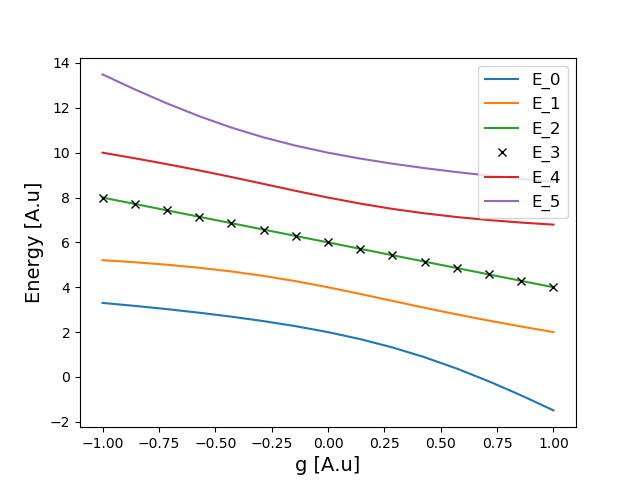
\includegraphics[width=0.7\textwidth]{eigval_vs_g.png}
\caption{The energy levels as a function of the strength $g$ for the analytic case of the pairing model. }
\label{fig: g_vs_eigval}
\end{figure}

In figure \ref{fig: g_vs_eigval} we see the eigenvalues of the Hamiltonian matrix \eqref{eq: analytic_H_matrix} for the pairing model as a function of the strength $g \in [-1,1]$. (The diagonalization was done with numpy)

-->Comment the behavior of the ground state as function of g?


%------------------------------------------------

\section{Discussion}



\section{Conclusions}

Structure of report (crude first idea):
\begin{enumerate}
\item Title
\item Abstract
\item Introduction
\begin{itemize}
\item Why useful
\item Where useful (nuc. chart)
\end{itemize}
\item The Pairing problem
\begin{itemize}
\item theory
\item analytic / exact results
\end{itemize}
\item Building a shell-model code
\begin{itemize}
\item Describe the different parts/blocks of the code (basis, SD, states, int, hamiltonian...)
\item Unit tests / benchmarks (analytic/exact results)
\item Psedo code?
\item Accuracy of our code
\item Where our code fails, why and proposing solutions
\end{itemize}
\item NuShellX
\begin{itemize}
\item describe why useful / 'powerful tool' and what may be calculated
\item compare with our own code
\item Possible 'future calculations'
\end{itemize}
\item Conclusions / Summary
\end{enumerate}


%----------------------------------------------------------------------------------------
%	REFERENCE LIST
%----------------------------------------------------------------------------------------

\begin{thebibliography}{99} % Bibliography - this is intentionally simple in this template
%
%\bibitem[Figueredo and Wolf, 2009]{Figueredo:2009dg}
%Figueredo, A.~J. and Wolf, P. S.~A. (2009).
%\newblock Assortative pairing and life history strategy - a cross-cultural
%  study.
%\newblock {\em Human Nature}, 20:317--330.

\bibitem[Github of the TALENT School][ MHJ and Alex Brown
\newblock {\em link goes here},
 
\end{thebibliography}

%----------------------------------------------------------------------------------------

\end{document}
